% M6-v0: không khóa, memset trước free (CÓ LỖI)
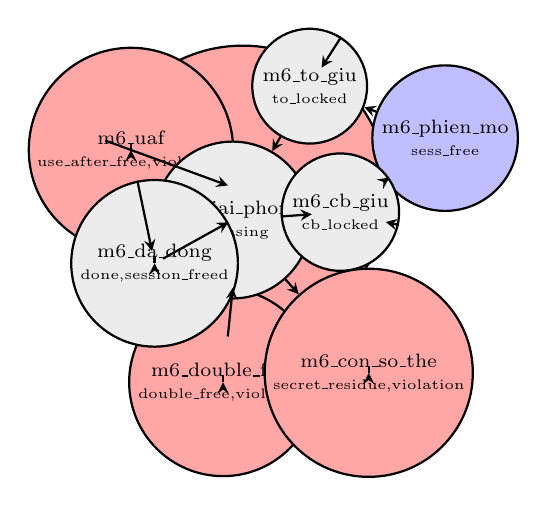
\begin{tikzpicture}[
  every node/.style={draw, circle, inner sep=2pt,
      minimum size=8mm, align=center, font=\scriptsize},
  ->, >=stealth, thick, auto
]
  \node[fill=red!35] (nd_m6_tranh_chap) at (-0.37,0.42) {m6\_tranh\_chap\\{\tiny cb\_locked,race,to\_locked,violation}};
  \node[fill=blue!25] (nd_m6_phien_mo) at (2.20,1.09) {m6\_phien\_mo\\{\tiny sess\_free}};
  \node[fill=red!35] (nd_m6_double_free) at (-0.62,-2.01) {m6\_double\_free\\{\tiny double\_free,violation}};
  \node[fill=red!35] (nd_m6_uaf) at (-1.79,0.94) {m6\_uaf\\{\tiny use\_after\_free,violation}};
  \node[fill=gray!15] (nd_m6_to_giu) at (0.48,1.75) {m6\_to\_giu\\{\tiny to\_locked}};
  \node[fill=gray!15] (nd_m6_giai_phong) at (-0.50,0.05) {m6\_giai\_phong\\{\tiny releasing}};
  \node[fill=gray!15] (nd_m6_cb_giu) at (0.87,0.15) {m6\_cb\_giu\\{\tiny cb\_locked}};
  \node[fill=red!35] (nd_m6_con_so_the) at (1.23,-1.89) {m6\_con\_so\_the\\{\tiny secret\_residue,violation}};
  \node[fill=gray!15] (nd_m6_da_dong) at (-1.49,-0.50) {m6\_da\_dong\\{\tiny done,session\_freed}};
  \draw (nd_m6_tranh_chap) -- (nd_m6_uaf);
  \draw (nd_m6_tranh_chap) -- (nd_m6_double_free);
  \draw (nd_m6_phien_mo) -- (nd_m6_to_giu);
  \draw (nd_m6_phien_mo) -- (nd_m6_cb_giu);
  \draw (nd_m6_double_free) -- (nd_m6_double_free);
  \draw (nd_m6_uaf) -- (nd_m6_uaf);
  \draw (nd_m6_to_giu) -- (nd_m6_giai_phong);
  \draw (nd_m6_to_giu) -- (nd_m6_tranh_chap);
  \draw (nd_m6_giai_phong) -- (nd_m6_con_so_the);
  \draw (nd_m6_giai_phong) -- (nd_m6_da_dong);
  \draw (nd_m6_cb_giu) -- (nd_m6_giai_phong);
  \draw (nd_m6_cb_giu) -- (nd_m6_tranh_chap);
  \draw (nd_m6_con_so_the) -- (nd_m6_con_so_the);
  \draw (nd_m6_da_dong) -- (nd_m6_uaf);
  \draw (nd_m6_da_dong) -- (nd_m6_da_dong);
\end{tikzpicture}

% M6-v1: mutex + status CLOSED + explicit_bzero
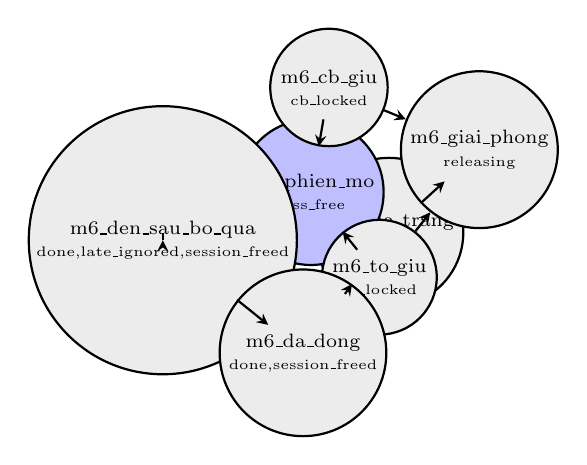
\begin{tikzpicture}[
  every node/.style={draw, circle, inner sep=2pt,
      minimum size=8mm, align=center, font=\scriptsize},
  ->, >=stealth, thick, auto
]
  \node[fill=gray!15] (nd_m6_xoa_trang) at (0.67,-0.17) {m6\_xoa\_trang\\{\tiny wiped}};
  \node[fill=blue!25] (nd_m6_phien_mo) at (-0.32,0.34) {m6\_phien\_mo\\{\tiny sess\_free}};
  \node[fill=gray!15] (nd_m6_to_giu) at (0.55,-0.74) {m6\_to\_giu\\{\tiny to\_locked}};
  \node[fill=gray!15] (nd_m6_den_sau_bo_qua) at (-2.20,-0.27) {m6\_den\_sau\_bo\_qua\\{\tiny done,late\_ignored,session\_freed}};
  \node[fill=gray!15] (nd_m6_giai_phong) at (1.82,0.88) {m6\_giai\_phong\\{\tiny releasing}};
  \node[fill=gray!15] (nd_m6_cb_giu) at (-0.09,1.67) {m6\_cb\_giu\\{\tiny cb\_locked}};
  \node[fill=gray!15] (nd_m6_da_dong) at (-0.42,-1.70) {m6\_da\_dong\\{\tiny done,session\_freed}};
  \draw (nd_m6_xoa_trang) -- (nd_m6_da_dong);
  \draw (nd_m6_phien_mo) -- (nd_m6_to_giu);
  \draw (nd_m6_phien_mo) -- (nd_m6_cb_giu);
  \draw (nd_m6_to_giu) -- (nd_m6_giai_phong);
  \draw (nd_m6_den_sau_bo_qua) -- (nd_m6_den_sau_bo_qua);
  \draw (nd_m6_giai_phong) -- (nd_m6_xoa_trang);
  \draw (nd_m6_cb_giu) -- (nd_m6_giai_phong);
  \draw (nd_m6_da_dong) -- (nd_m6_den_sau_bo_qua);
\end{tikzpicture}